\chapter{Experimentos e Resultados Preliminares}\label{cap:experimentos}

\section{Base de dados}

A base de dados (imagens) utilizada advém do projeto GEOMA \cite{geoma}, financiado pelo Instituto de Pesquisas Espaciais (INPE). Trata-se de imagens coloridas, codificadas em JPEG e com 640 pixels de largura por 480 pixels de altura. A base é composta por fotografias ortogonais ao relevo (como pode ser visto na figura \ref{fig:amostra}), de altitudes variadas e tiradas a partir de aeronaves tripuladas, durante o trajeto entre diversas cidades da região amazônica.

No momento do início dos experimentos deste trabalho, estas imagens tiradas de aviões tripulados eram as únicas disponíveis publicamente. Podemos considerá-las válidas por terem sido tiradas em altitude de vôo compatível com as missões de VANTs de vigilância, entre 900 e 1.100 metros do solo. Como este trabalho tem como objetivo utilizar apenas câmeras de espectro visível, são dispensáveis comparações de sensores com VANTs que eventualmente possuam sonar, câmeras infravermelho ou outros tipos de sensores.

\begin{figure}[h]
  \centering
  \begin{subfigure}[b]{0.3\textwidth}
    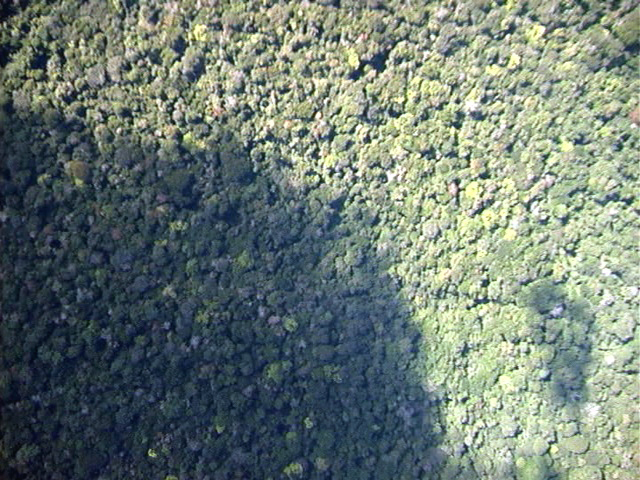
\includegraphics[width=\textwidth]{imgs/amostra1}
  \end{subfigure}%
  ~
  \begin{subfigure}[b]{0.3\textwidth}
    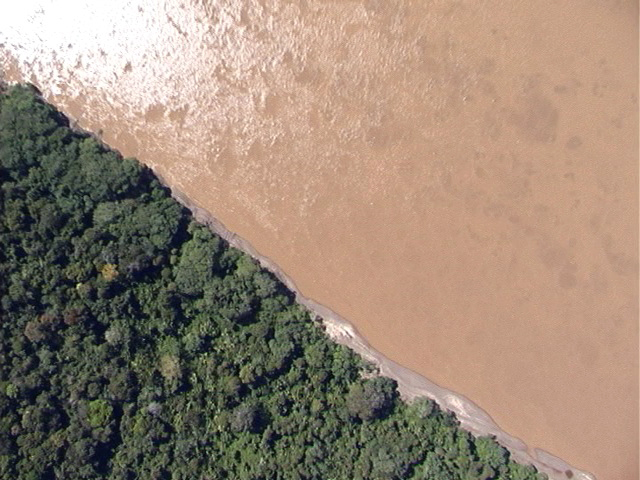
\includegraphics[width=\textwidth]{imgs/amostra2}
  \end{subfigure}%
  ~
  \begin{subfigure}[b]{0.3\textwidth}
    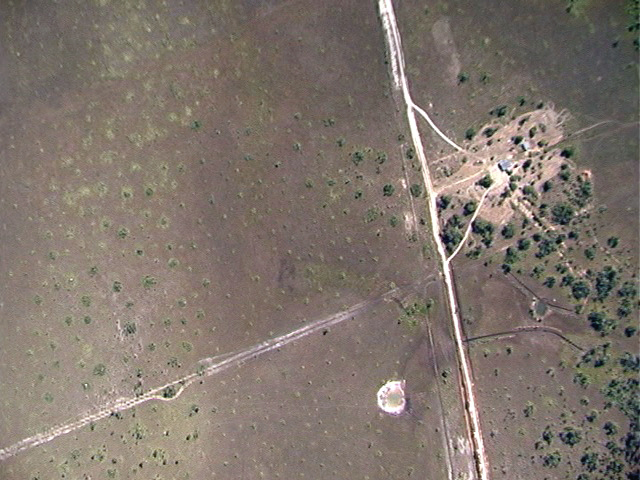
\includegraphics[width=\textwidth]{imgs/amostra3}
  \end{subfigure}%
  \caption{Amostras da base de dados}
  \label{fig:amostra}
\end{figure}

A base possui um total de 3.044 imagens, com dimensão total de 1,02 Gigabytes de dados. Cerca de 150 imagens foram utilizadas nos experimentos até o momento, visto que um grande esforço precisa ser despendido na classificação manual das imagens em todas as etapas do experimento, consumindo um tempo considerável.

Para facilitar a classificação manual foi construída uma ferramenta gráfica que permite ao usuário segmentar e classificar as regiões das imagens de acordo com as classes disponíveis (figura \ref{fig:visualClassifier}). A saída deste aplicativo é uma coleção, para cada imagem, de informações sobre bordas das regiões e a classificação de cada pixel. Posteriormente essas informações serão confrontadas com o resultado da segmentação e primeiro nível de classificação da solução.

\begin{figure}[h]
  \centering
  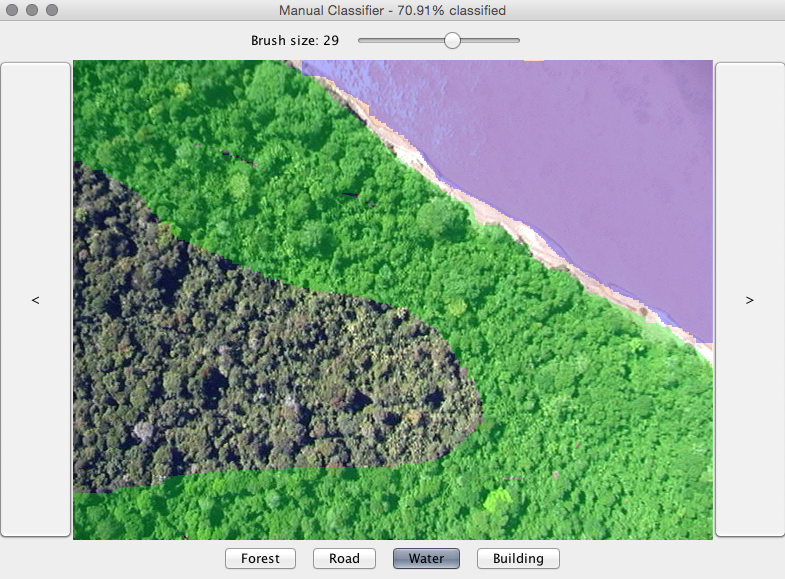
\includegraphics[width=0.7\textwidth]{imgs/visualClassifier}
  \caption{Ferramenta para segmentação e classificação manual das imagens em regiões}
  \label{fig:visualClassifier}
\end{figure}

\section{Segmentação}

\section{Classificações de regiões}

\section{Próximos passos}
